% Informe técnico del Proyecto 2 (CC3074 Modelación y Simulación, UVG).
% Compilar con XeLaTeX:   cd report && latexmk -xelatex main.tex
% Las cifras y tablas se importan de Output/report/generated/, que produce
% Output/scripts/build_report_assets.py a partir de evidence/final/.
\documentclass[11pt,a4paper]{article}

\usepackage{fontspec}
\usepackage[provide=*,main=spanish]{babel}
\usepackage[margin=2.5cm]{geometry}
\usepackage{microtype}
\usepackage{amsmath,amssymb}
\usepackage{booktabs,tabularx,array}
\usepackage{graphicx}
\usepackage{caption}
\usepackage{enumitem}
\usepackage{tikz}
\usetikzlibrary{arrows.meta,positioning,shapes.geometric}
\usepackage[most]{tcolorbox}
\usepackage[numbers,sort&compress]{natbib}
\usepackage[hidelinks]{hyperref}

\setlist{itemsep=2pt,topsep=4pt}
\captionsetup{font=small,labelfont=bf}
\captionsetup[table]{name=Tabla}
\setcounter{tocdepth}{1}
\setlength{\parskip}{4pt}
\setlength{\emergencystretch}{3em}
\setlength{\parindent}{0pt}
\renewcommand{\arraystretch}{1.12}

% Cuadro de alcance de la afirmación (se repite cerca de los resultados).
\newtcolorbox{alcance}[1][Alcance de la afirmación]{
  colback=gray!8,colframe=gray!60!black,fonttitle=\bfseries\small,
  title=#1,boxrule=0.6pt,arc=2pt,left=6pt,right=6pt,top=4pt,bottom=4pt}

% Tablas anchas: letra pequeña y escalado al ancho de página.
\newcommand{\fittable}[1]{\begin{center}\small\resizebox{\linewidth}{!}{\input{#1}}\end{center}}

% Generado por scripts/build_report_assets.py. No editar a mano.
\newcommand{\NReps}{30}
\newcommand{\NRuns}{180}
\newcommand{\NConditions}{6}
\newcommand{\OptSeedFirst}{10000}
\newcommand{\OptSeedLast}{10009}
\newcommand{\EvalSeedFirst}{30000}
\newcommand{\EvalSeedLast}{30029}
\newcommand{\AlgSeed}{9101}
\newcommand{\GitCommit}{8c7685a}
\newcommand{\PythonVersion}{3.13.17}
\newcommand{\AllDrained}{sí}
\newcommand{\MaxNotStarted}{0}
\newcommand{\WaitBaseLow}{22.87}
\newcommand{\WaitCandLow}{21.05}
\newcommand{\RedLow}{1.81}
\newcommand{\RedPctLow}{7.9}
\newcommand{\RedCILowLow}{$-$6.96}
\newcommand{\RedCIHighLow}{10.59}
\newcommand{\PairsPosLow}{12}
\newcommand{\DrainBaseLow}{17.1}
\newcommand{\DrainCandLow}{18.5}
\newcommand{\WaitBaseNom}{74.52}
\newcommand{\WaitCandNom}{53.60}
\newcommand{\RedNom}{20.92}
\newcommand{\RedPctNom}{28.1}
\newcommand{\RedCILowNom}{9.11}
\newcommand{\RedCIHighNom}{32.73}
\newcommand{\PairsPosNom}{21}
\newcommand{\DrainBaseNom}{83.8}
\newcommand{\DrainCandNom}{89.8}
\newcommand{\WaitBaseHigh}{228.09}
\newcommand{\WaitCandHigh}{177.32}
\newcommand{\RedHigh}{50.76}
\newcommand{\RedPctHigh}{22.3}
\newcommand{\RedCILowHigh}{37.02}
\newcommand{\RedCIHighHigh}{64.50}
\newcommand{\PairsPosHigh}{26}
\newcommand{\DrainBaseHigh}{382.3}
\newcommand{\DrainCandHigh}{372.8}
\newcommand{\NomBaseMedian}{27.54}
\newcommand{\NomCandMedian}{15.90}
\newcommand{\NomRedMedian}{11.64}
\newcommand{\NomRedPctMedian}{42.3}
\newcommand{\NomBasePninety}{236.69}
\newcommand{\NomCandPninety}{158.84}
\newcommand{\NomRedPninety}{77.86}
\newcommand{\NomRedPctPninety}{32.9}
\newcommand{\NomBaseShare}{0.271}
\newcommand{\NomCandShare}{0.225}
\newcommand{\NomRedShare}{0.047}
\newcommand{\NomRedPctShare}{17.2}
\newcommand{\NomBaseQueue}{3.72}
\newcommand{\NomCandQueue}{2.63}
\newcommand{\NomRedQueue}{1.09}
\newcommand{\NomRedPctQueue}{29.4}
\newcommand{\StdBaseNom}{60.59}
\newcommand{\StdCandNom}{49.94}
\newcommand{\MargBaseLow}{52.84}
\newcommand{\MargBaseHigh}{96.20}
\newcommand{\MargCandLow}{35.73}
\newcommand{\MargCandHigh}{71.47}
\newcommand{\RefMeanWait}{38.15}
\newcommand{\RefMedianWait}{16.00}
\newcommand{\RefPninetyWait}{98.00}
\newcommand{\RefShare}{0.177}
\newcommand{\RefMeanCILow}{32.34}
\newcommand{\RefMeanCIHigh}{43.97}
\newcommand{\RefN}{13\,272}
\newcommand{\MedianCandErr}{0.10}
\newcommand{\PninetyCandErr}{60.84}
\newcommand{\MaeBase}{62.20}
\newcommand{\MaeCand}{25.46}
\newcommand{\MaePropBase}{0.094}
\newcommand{\MaePropCand}{0.048}
\newcommand{\OptBaseWait}{85.44}
\newcommand{\OptCandWait}{49.67}
\newcommand{\OptObjBase}{134.58}
\newcommand{\OptObjCand}{76.92}
\newcommand{\OptRelPct}{42.8}
\newcommand{\OptEvaluated}{61}
\newcommand{\OptGenerations}{9}
\newcommand{\DailyVolume}{63.98}
\newcommand{\DailyVolumeRound}{64}
\newcommand{\ServiceSigma}{0.45}


\title{Redistribución horaria de equipos de atención en un departamento de
emergencias de referencia:\\ simulación de eventos discretos y algoritmo genético restringido}
\author{Pablo Daniel Barillas Moreno \and Jorge Palacios \and
Adrián Ricardo González Muralles \and Andrés Rafael Chivalán \and
Javier Andrés Chen}
\date{Universidad del Valle de Guatemala\\
CC3074 Modelación y Simulación, sección 30 --- Proyecto 2, Grupo 1\\
Noviembre de 2026}

\begin{document}
\maketitle
\thispagestyle{empty}

\begin{abstract}
\noindent
Este informe estudia si redistribuir una cantidad fija de equipos de atención entre
seis bloques de cuatro horas reduce la espera de los pacientes de un departamento de
emergencias (DE) de referencia, sin aumentar las horas-equipo. Se construyó una
simulación de eventos discretos (SimPy) con llegadas dependientes de la hora, cola
no expropiativa con prioridad de triaje y capacidad variable, calibrada con el archivo
público NHAMCS 2022 de los CDC. Un algoritmo genético con restricciones propuso un
horario candidato (1, 2, 5, 5, 6, 4 equipos frente a 3, 3, 4, 4, 5, 4 del horario base,
ambos con 23 unidades).
Se evaluó con \NReps{} réplicas independientes por condición, con semillas pareadas
y distintas de las usadas para optimizar. Bajo la demanda nominal, la espera media
simulada pasó de \WaitBaseNom{} a \WaitCandNom{} min (reducción pareada de \RedNom{} min,
\RedPctNom\,\%; IC 95\,\% [\RedCILowNom, \RedCIHighNom] min). El efecto es incierto
con demanda baja y mayor con demanda alta. La mejora es \emph{simulada}, no observada;
el modelo base sobreestima las esperas de NHAMCS y no representa a un hospital
guatemalteco.
\end{abstract}

\newpage
\tableofcontents
\newpage

\section*{Resumen ejecutivo}
\addcontentsline{toc}{section}{Resumen ejecutivo}

\textbf{Pregunta.} ¿Cuánto puede reducirse la espera hasta el inicio de la atención al
redistribuir 23 unidades de capacidad (92 horas-equipo diarias) entre seis bloques de
cuatro horas, sin aumentar el total?

\textbf{Qué se hizo.} Se simuló un DE de referencia (la mediana de volumen de los DE de
NHAMCS 2022) y se buscó con un algoritmo genético restringido un horario que minimiza una
combinación de espera media y percentil 90. Se congeló la candidata con semillas de
optimización (\OptSeedFirst--\OptSeedLast) y se evaluó con otras
(\EvalSeedFirst--\EvalSeedLast): \NConditions{} condiciones (2 horarios $\times$ 3 niveles
de demanda), \NReps{} réplicas por condición, \NRuns{} ejecuciones en total.

\textbf{Qué mejoró y cuánto.}
\begin{itemize}
  \item \emph{Demanda nominal:} espera media de \WaitBaseNom{} a \WaitCandNom{} min,
  una reducción pareada de \RedNom{} min (\RedPctNom\,\%), IC 95\,\% [\RedCILowNom,
  \RedCIHighNom] min; mediana de \NomBaseMedian{} a \NomCandMedian{} min, percentil 90 de
  \NomBasePninety{} a \NomCandPninety{} min y proporción con espera $>$ 60 min de
  \NomBaseShare{} a \NomCandShare{}. El horario candidato favorece a \PairsPosNom{} de
  las \NReps{} parejas.
  \item \emph{Demanda alta (1.20):} reducción de \RedHigh{} min (\RedPctHigh\,\%), IC 95\,\%
  [\RedCILowHigh, \RedCIHighHigh] min.
  \item \emph{Demanda baja (0.80):} reducción de \RedLow{} min con IC 95\,\% [\RedCILowLow,
  \RedCIHighLow] min, que incluye el cero; no se afirma mejora en esa condición.
\end{itemize}

\textbf{Qué tan confiable es la comparación.} La comparación entre horarios es pareada
(mismas semillas) y descrita con intervalos, pero la variación entre días simulados es
grande (desviación estándar de la espera media nominal: \StdBaseNom{} min en la base y
\StdCandNom{} min en la candidata). Frente a la espera observada en NHAMCS
(\RefMeanWait{} min), el modelo base la sobreestima (\WaitBaseNom{} min); la candidata se
acerca (\WaitCandNom{} min), pero eso no valida la intervención, porque el algoritmo no se
ajustó a \texttt{WAITTIME}.

\textbf{Limitaciones principales.} El tiempo de servicio es un supuesto, no un dato
observado; el modelo usa un recurso único agregado sin preempción ni abandono; NHAMCS es
una referencia nacional de Estados Unidos y no describe un hospital guatemalteco; con
demanda alta el sistema se satura (drenajes medios de \DrainBaseHigh{}--\DrainCandHigh{}~min).

\begin{alcance}
La mejora que se reporta es una \textbf{mejora simulada} bajo supuestos explícitos. No se
implementó ninguna intervención ni se observó una mejora clínica u operativa real.
\end{alcance}

\newpage

\section{Problema real, contexto, objetivo y pregunta}

\subsection{Contexto}
Los departamentos de emergencias reciben una demanda que cambia con la hora, mientras que
la capacidad suele asignarse por turnos de forma más rígida. Una distribución uniforme de
equipos puede dejar capacidad ociosa en horas tranquilas y formar colas en horas de mayor
llegada. El proyecto evalúa, mediante simulación, si reasignar la \emph{misma} cantidad de
recursos entre bloques horarios reduce el tiempo de espera.

El escenario de referencia es un DE estadounidense descrito por datos públicos de NHAMCS
2022 \citep{nhamcs2022doc}. No pretende caracterizar un hospital en particular ni producir
recomendaciones clínicas.

\subsection{Pregunta de investigación}
\begin{quote}
\emph{¿Cuánto puede reducirse el tiempo de espera de los pacientes al redistribuir una
cantidad fija de equipos de atención entre seis bloques de cuatro horas, sin aumentar las
horas-recurso totales?}
\end{quote}

\subsection{Objetivos}
\textbf{General.} Diseñar, implementar y evaluar una simulación de eventos discretos que
compare una asignación base con una asignación optimizada de recursos.

\textbf{Específicos.}
\begin{enumerate}
  \item Estimar perfiles horarios de llegada y de triaje con datos públicos NHAMCS 2022.
  \item Construir un modelo parametrizable con llegadas aleatorias, prioridades y capacidad
  variable.
  \item Implementar un algoritmo genético que redistribuya recursos sin aumentar el total.
  \item Verificar automáticamente que toda solución propuesta cumpla las restricciones.
  \item Comparar escenarios con métricas comunes, semillas pareadas y una referencia real.
\end{enumerate}

\subsection{Métricas}
La métrica principal es la \textbf{espera media hasta el inicio de la atención}, en
minutos, con sentido de minimización. Las métricas secundarias son la mediana, el
percentil 90, la proporción de pacientes con espera superior a 60 minutos, la cola media y
máxima (pacientes) y la utilización de los equipos (proporción).

\subsection{Alcance y supuestos}
\begin{itemize}
  \item Horizonte de 24 horas en seis bloques de cuatro horas; la capacidad solo cambia al
  inicio de cada bloque.
  \item Cada paciente usa un solo equipo a la vez; el nivel de triaje no cambia durante la
  espera.
  \item La cola respeta prioridad clínica y, dentro de cada prioridad, el orden de llegada.
  \item El servicio es una abstracción de ocupación del equipo, no tiempo continuo de
  contacto con un médico.
  \item Quedan fuera: diagnóstico y resultados clínicos, traslados, disponibilidad
  individual de personal, camas de hospitalización y cualquier predicción para Guatemala.
\end{itemize}

\section{Fuente pública y clasificación de datos}

\subsection{NHAMCS 2022}
La referencia es el archivo público de visitas a departamentos de emergencias de la
\emph{National Hospital Ambulatory Medical Care Survey} 2022, publicado por el National
Center for Health Statistics (NCHS) de los CDC
\citep{nhamcs2022doc,nhamcs2022data,nhamcs2022dictionary}. El archivo contiene 16\,025
visitas en 188 departamentos y representa, con pesos muestrales, 155\,397\,747 visitas;
cada hospital reporta durante un periodo de cuatro semanas asignado al azar dentro de 2022.
El procedimiento de descarga verifica tamaño y suma de verificación (SHA-256) y consta en
el repositorio (\texttt{data/README.md}, \texttt{docs/05\_data\_calibration.md}). Los
resúmenes nacionales oficiales se consultan en \citet{nhamcs2022tables}.

Las variables usadas son:
\begin{itemize}
  \item \texttt{ARRTIME}: hora de llegada (perfil horario);
  \item \texttt{IMMEDR}: urgencia recomendada, niveles 1--5 (probabilidades de triaje);
  \item \texttt{PATWT} y \texttt{EDWT}: pesos de visita y de departamento (ponderación y
  volumen por departamento);
  \item \texttt{WAITTIME}: minutos hasta el primer contacto con médico, APRN o PA
  (\emph{referencia de validación});
  \item \texttt{LOV} y \texttt{BOARDED}: duración de la visita y tiempo de \emph{boarding}
  (solo para acotar el servicio, ver sección~\ref{sec:calibracion}).
\end{itemize}

El archivo crudo no se versiona: el \emph{readme} oficial restringe su uso a fines
estadísticos \citep{nhamcs2022readme}. El repositorio publica únicamente agregados.

\subsection{Clasificación de los valores publicados}
Todo valor que aparece en el informe lleva una de cuatro etiquetas de procedencia
(tabla~\ref{tab:procedencia}).

\begin{table}[ht]
\centering\small
\caption{Categorías de procedencia usadas en el proyecto.}
\label{tab:procedencia}
\begin{tabularx}{\linewidth}{@{}l X X@{}}
\toprule
Etiqueta & Significado & Ejemplo en este proyecto \\
\midrule
\texttt{observed\_public} & Observado en una fuente pública & Registros individuales de NHAMCS (no se publican sin agregar) \\
\texttt{derived\_from\_public} & Calculado a partir de datos públicos & Perfil horario, probabilidades de triaje, volumen diario, espera de referencia \\
\texttt{estimated\_assumption} & Supuesto o estimación del equipo & Medianas y $\sigma$ de servicio, presupuesto de 23 unidades, límites del horario \\
\texttt{synthetic\_simulation} & Generado por el modelo & Llegadas, esperas, colas y utilización simuladas \\
\bottomrule
\end{tabularx}
\end{table}

\begin{alcance}
NHAMCS es una referencia pública nacional de Estados Unidos. No representa a un hospital
guatemalteco específico ni autoriza a afirmar que una intervención se aplicó o produjo una
mejora real.
\end{alcance}

\section{Investigación: simulación, algoritmo genético y alternativas}

\subsection{Simulación de eventos discretos}
El estado de un DE cambia en instantes discretos (llegada, inicio y fin de atención), y la
congestión surge de la interacción entre llegadas aleatorias y capacidad limitada. La
simulación de eventos discretos (DES) avanza el reloj solo entre eventos y permite registrar
cada espera y comparar políticas bajo las mismas secuencias aleatorias. Se usó SimPy
\citep{simpy412} para el reloj, la agenda de eventos y los recursos con prioridad; el
equipo desarrolló los procesos de paciente, el cambio de capacidad por bloque, la cola
clínica, las métricas y las verificaciones.

\subsection{Algoritmo genético restringido}
Un algoritmo genético (GA) mantiene una población de soluciones y las mejora mediante
selección, cruce y mutación \citep{eiben2015evolutionary}. Aquí un individuo es un vector
entero $x=(x_0,\dots,x_5)$ con los equipos de cada bloque de cuatro horas. La evaluación
de un individuo es una simulación estocástica, por lo que el GA usa la DES como función de
aptitud ruidosa. Las restricciones se manejan con la regla de factibilidad de
\citet{deb2000constraints}: una solución factible domina a una no factible; entre factibles
gana el menor objetivo; entre no factibles gana la menor violación. La literatura reciente
sobre dotación de personal en emergencias combina simulación y optimización de forma
similar \citep{wang2025staffing}.

\subsection{Alternativas consideradas}
\begin{table}[ht]
\centering\small
\caption{Comparación de técnicas de optimización para el problema de dotación horaria.}
\label{tab:alternativas}
\begin{tabularx}{\linewidth}{@{}l X X@{}}
\toprule
Alternativa & Ventaja & Por qué no es la técnica principal \\
\midrule
Enumeración exhaustiva & Encuentra el mejor valor del espacio evaluado & Cada candidato exige varias simulaciones; el costo crece con límites, bloques y réplicas \\
Programación lineal entera & Ofrece garantías en problemas lineales & La espera y sus percentiles emergen de una simulación no lineal y estocástica \\
Búsqueda aleatoria & Sencilla; útil como referencia & No reutiliza información de soluciones prometedoras \\
Enjambre de partículas & Buen desempeño en espacios continuos & Representación entera, restringida, con reparación frecuente \\
Algoritmo genético & Maneja vectores enteros, operadores propios y restricciones & No garantiza optimalidad global; exige controlar ruido y convergencia \\
\bottomrule
\end{tabularx}
\end{table}

\subsection{Limitaciones de la técnica}
Un GA no demuestra optimalidad global y puede converger prematuramente. Con pocas
réplicas por candidato puede seleccionar por ruido; por eso la candidata se reevalúa con
semillas independientes (sección~\ref{sec:diseno}). La investigación previa del proyecto
planteó una búsqueda aleatoria con el mismo presupuesto de evaluaciones como comparador;
\emph{la evidencia final no incluye ese comparador}, de modo que no se puede afirmar cuánto
aporta la estructura evolutiva frente a probar horarios al azar.

\section{Formulación matemática y diagrama del modelo}
\label{sec:formulacion}

\subsection{Diagrama del sistema}
\begin{figure}[ht]
\centering
\resizebox{\linewidth}{!}{%
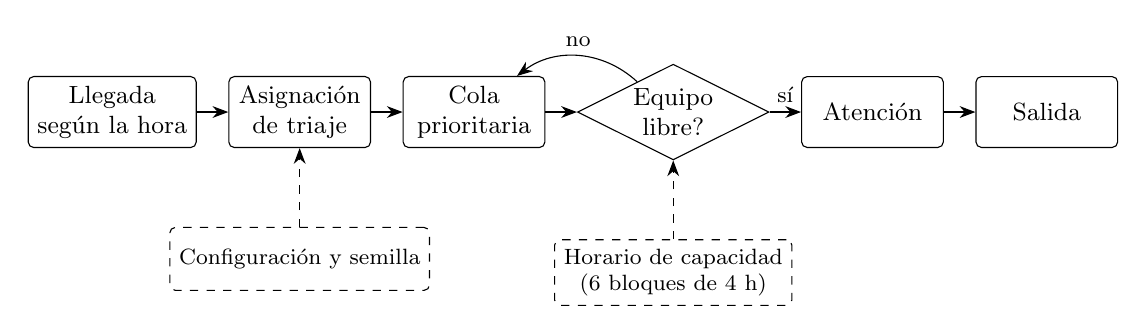
\begin{tikzpicture}[
  node distance=4mm and 4mm,
  box/.style={draw,rounded corners=2pt,minimum height=9mm,minimum width=18mm,align=center,font=\small},
  dec/.style={draw,diamond,aspect=2,inner sep=1pt,align=center,font=\small},
  param/.style={draw,dashed,rounded corners=2pt,minimum height=8mm,align=center,font=\footnotesize},
  >={Stealth[length=2mm]}]
  \node[box] (arr) {Llegada\\según la hora};
  \node[box,right=of arr] (tri) {Asignación\\de triaje};
  \node[box,right=of tri] (cola) {Cola\\prioritaria};
  \node[dec,right=of cola] (dis) {Equipo\\libre?};
  \node[box,right=of dis] (ate) {Atención};
  \node[box,right=of ate] (sal) {Salida};
  \node[param,below=10mm of dis] (cap) {Horario de capacidad\\(6 bloques de 4 h)};
  \node[param,below=10mm of tri] (cfg) {Configuración y semilla};
  \draw[->] (arr)--(tri); \draw[->] (tri)--(cola); \draw[->] (cola)--(dis);
  \draw[->] (dis)--node[above,font=\footnotesize]{sí}(ate); \draw[->] (ate)--(sal);
  \draw[->] (dis) to[bend right=40] node[above,font=\footnotesize]{no} (cola);
  \draw[->,dashed] (cap)--(dis);
  \draw[->,dashed] (cfg)--(tri);
\end{tikzpicture}}
\caption{Flujo del paciente en el modelo. La capacidad por bloque determina cuántas
atenciones pueden ejecutarse simultáneamente; la semilla controla llegadas, triaje y
duración.}
\label{fig:sistema}
\end{figure}

\subsection{Variables y parámetros}
\begin{table}[ht]
\centering\small
\caption{Variables del modelo, unidades y procedencia.}
\label{tab:variables}
\begin{tabularx}{\linewidth}{@{}l l l X l@{}}
\toprule
Símbolo & Tipo & Unidad & Descripción & Procedencia \\
\midrule
$\lambda_h$ & Parámetro & pac./h & Tasa de llegada en la hora $h$ & derivado \\
$p_k$ & Parámetro & proporción & Probabilidad del triaje $k=1,\dots,5$ & derivado \\
$m_k,\ \sigma$ & Parámetro & min, --- & Mediana y dispersión lognormal del servicio & supuesto \\
$x_b$ & Decisión & equipos & Capacidad del bloque $b=0,\dots,5$ & supuesto / GA \\
$Q(t)$ & Estado & pacientes & Cola física completa & simulado \\
$B(t)$ & Estado & equipos & Equipos atendiendo & simulado \\
$W_i$ & Salida & min & Inicio de servicio menos llegada del paciente $i$ & simulado \\
$U$ & Salida & proporción & Utilización efectiva de los equipos & simulado \\
\bottomrule
\end{tabularx}
\end{table}

\subsection{Llegadas}
En cada hora se supone una tasa constante $\lambda_h=V\,p_h$, con $p_h$ la proporción
ponderada de llegadas en la hora $h$ y $V$ el volumen diario de referencia. El tiempo entre
llegadas es
\begin{equation}
T_h=-\frac{\ln U}{\lambda_h},\qquad U\sim\mathrm{Uniforme}(0,1),
\end{equation}
y si el tiempo generado cruza la frontera horaria, el reloj avanza hasta la frontera y se
vuelve a muestrear con la nueva tasa. Es una aproximación por tramos de un proceso de
Poisson no homogéneo.

\subsection{Prioridad y servicio}
Los niveles de triaje van de 1 (mayor urgencia) a 5. La cola es no expropiativa: una
atención en curso no se interrumpe cuando llega un paciente más urgente; la prioridad solo
ordena a los pacientes en espera, y a igual prioridad se respeta el orden de llegada. La
duración de la atención del nivel $k$ es lognormal acotada:
\begin{equation}
S_k\sim\mathrm{Lognormal}\bigl(\ln m_k,\ \sigma\bigr).
\end{equation}

\subsection{Capacidad variable, calentamiento y drenaje}
El recurso se crea con la capacidad máxima diaria y controladores bloquean los espacios no
disponibles en cada bloque. Si la capacidad baja, la atención en curso termina y luego el
espacio se bloquea, de modo que nadie es expulsado del servicio. La utilización se define
sobre la capacidad \emph{efectiva} (la que los pacientes pueden usar):
\begin{equation}
U=\frac{\text{minutos-equipo ocupados en la ventana}}
       {\text{minutos-equipo efectivos disponibles en la ventana}}\ \le 1.
\end{equation}

Cada ejecución simula dos días: el primero es calentamiento y el segundo es la ventana de
medición. Los pacientes que llegaron durante el calentamiento y siguen esperando
permanecen en la cola física y cuentan desde el inicio de la medición; solo se reinician
los acumuladores estadísticos. Al terminar la ventana se detienen las llegadas y se
\emph{drena} la cohorte medida hasta que todos inician servicio, de modo que las esperas
son completas y no hay censura. El tiempo de drenaje se registra aparte y no entra en la
cola, capacidad ni utilización de la ventana.

\subsection{Función objetivo y restricciones}
Para un horario $x$ se minimiza
\begin{equation}
J(x)=0.7\,\overline{W}(x)+0.3\,Q_{0.90}\bigl(W(x)\bigr)+120\,C(x),
\end{equation}
con $\overline{W}$ la espera media (min), $Q_{0.90}$ el percentil 90 de la espera (min) y
$C$ la proporción de pacientes que no inició atención al final (el término evita premiar
colas sin atender; con el drenaje vale cero). Las restricciones son
\begin{equation}
x_b\in\mathbb{Z},\quad 1\le x_b\le 8,\quad \sum_{b=0}^{5}x_b=23,\quad
|x_{(b+1)\bmod 6}-x_b|\le 3.
\end{equation}
La suma fija conserva las 92 horas-equipo diarias porque los seis bloques duran lo mismo,
y la última restricción incluye la transición del último bloque al primero porque el
horario se repite cada día.

\section{Implementación del simulador y de la mejora}

\subsection{Organización del código}
El paquete \texttt{ed\_simulation} separa responsabilidades: \texttt{config.py}
(parámetros y validación temprana), \texttt{simulation.py} (procesos y métricas),
\texttt{calibration.py} (datos NHAMCS), \texttt{optimization/} (GA y restricciones),
\texttt{experiments.py}, \texttt{validation.py} y \texttt{evidence.py} (diseño
experimental, comparación con la referencia y figuras), \texttt{cli.py} (ejecución
reproducible) y \texttt{ui/} junto con \texttt{app.py} (interfaz Streamlit). La interfaz y
la CLI usan las mismas funciones públicas del simulador y del optimizador.

\subsection{Integración del algoritmo genético con la simulación}
El optimizador no modifica la simulación: para cada horario crea una configuración nueva
y la evalúa con el mismo modelo que usan la CLI y la interfaz. Todos los candidatos de una
búsqueda se evalúan con el mismo conjunto de semillas (números aleatorios comunes), lo que
reduce el ruido al compararlos.

\begin{itemize}
  \item \textbf{Inicialización:} la población incluye el horario base y recorridos
  aleatorios por vecinos factibles (transferir una unidad de un bloque a otro).
  \item \textbf{Selección:} torneo de tres con la regla de factibilidad de Deb.
  \item \textbf{Cruce y reparación:} cruce uniforme seguido de reparación determinista que
  limita valores, recupera el presupuesto y reduce violaciones de transición.
  \item \textbf{Mutación:} transferencia de una unidad entre dos bloques, aceptando solo
  vecinos factibles.
  \item \textbf{Elitismo y terminación:} dos élites pasan intactas; se detiene por máximo de
  generaciones o por falta de mejora durante la paciencia configurada.
\end{itemize}
Antes de devolver una solución se vuelve a comprobar que sea factible; de lo contrario el
programa falla en lugar de aceptarla.

\begin{table}[ht]
\centering\small
\caption{Configuración del algoritmo genético y de la búsqueda que congeló la candidata.}
\label{tab:ga}
\begin{tabular}{lr}
\toprule
Parámetro & Valor \\
\midrule
Población & 24 \\
Generaciones máximas & 20 \\
Probabilidad de cruce & 0.8 \\
Probabilidad de mutación & 0.25 \\
Élites & 2 \\
Tamaño de torneo & 3 \\
Paciencia (generaciones) & 8 \\
Réplicas por candidata & 10 \\
Semilla del algoritmo & 9101 \\
Horarios evaluados & 61 \\
Detención temprana & sí \\
\bottomrule
\end{tabular}

\end{table}

\subsection{Candidata obtenida}
La búsqueda usó diez réplicas por candidato con semillas \OptSeedFirst--\OptSeedLast{} y
semilla del algoritmo \AlgSeed. Evaluó \OptEvaluated{} horarios distintos y se detuvo
tras \OptGenerations{} generaciones por falta de mejora. El resultado se escribe en
\texttt{evidence/final/frozen\_candidate.json} \emph{antes} de la evaluación final.

\begin{table}[ht]
\centering\small
\caption{Horarios comparados (equipos por bloque de cuatro horas). Ambos suman 23
unidades (92 horas-equipo diarias) y cumplen todas las restricciones.}
\label{tab:horarios}
\begin{tabular}{lrrrrrrr}
\toprule
Horario & 00--04 & 04--08 & 08--12 & 12--16 & 16--20 & 20--24 & Total \\
\midrule
Base & 3 & 3 & 4 & 4 & 5 & 4 & 23 \\
Candidata congelada & 1 & 2 & 5 & 5 & 6 & 4 & 23 \\
\bottomrule
\end{tabular}

\end{table}

En el conjunto de optimización, el objetivo pasó de \OptObjBase{} a \OptObjCand{}
(\OptRelPct\,\% menos) y la espera media de \OptBaseWait{} a \OptCandWait{} min. Esa
mejora es mayor que la medida después con semillas independientes (sección~\ref{sec:resultados}):
parte de ella refleja la selección del mejor horario sobre un conjunto de semillas, lo que
justifica la evaluación independiente.

\subsection{Interpretación del horario}
La candidata reduce la capacidad en la madrugada (bloques 00--04 y 04--08) y la traslada a
la mañana, la tarde y el inicio de la noche (08--12, 12--16 y 16--20). Es coherente con
una demanda mayor durante el día, pero la lectura es descriptiva: el estudio no prueba por
qué ese vector particular es mejor que otros factibles.

\section{Calibración y procedencia de parámetros}
\label{sec:calibracion}

\subsection{Qué se calibra y qué se reserva para validar}
La calibración usa NHAMCS para tres entradas y reserva una cuarta variable para validar.
Si algún parámetro se ajustara para reproducir \texttt{WAITTIME}, esa validación dejaría de
ser independiente.

\begin{table}[ht]
\centering\small
\caption{Uso de las variables de NHAMCS 2022.}
\label{tab:usovars}
\begin{tabularx}{\linewidth}{@{}l l X@{}}
\toprule
Uso & Variables & Resultado \\
\midrule
Calibración & \texttt{ARRTIME} & Perfil horario de llegadas (derivado) \\
Calibración & \texttt{IMMEDR} & Probabilidades de triaje 1--5 (derivado) \\
Calibración & \texttt{PATWT}, \texttt{EDWT} & Volumen diario de un DE de referencia (derivado) \\
Validación & \texttt{WAITTIME} & Media, mediana, percentil 90 y proporción $>$ 60 min \\
Solo referencia & \texttt{LOV}, \texttt{BOARDED} & Cota superior de la ocupación de un equipo \\
\bottomrule
\end{tabularx}
\end{table}

\subsection{Perfil horario, triaje y volumen}
Las proporciones, medias y cuantiles usan \texttt{PATWT}; los errores estándar se obtienen
por linealización de Taylor con las variables de diseño enmascaradas de NCHS. Los códigos
especiales del libro de códigos (por ejemplo, ``en blanco'', ``no aplica'', ``desconocido'')
se convierten en faltantes y nunca se interpretan como cantidades clínicas; cada registro
se excluye solo de las estimaciones que requieren esa variable. Se asume que, tras
ponderar, los registros excluidos se parecen a los incluidos, supuesto relevante porque la
no respuesta documentada es de 27.8\,\% en \texttt{IMMEDR} y de 14.1\,\% en \texttt{WAITTIME}.

La tasa horaria es $\lambda_h=V\,p_h$. El perfil nacional indica \emph{cuándo} llegan los
pacientes, no \emph{cuántos} llegan a un hospital: por eso $V$ es una decisión separada. Se
tomó la \textbf{mediana de volumen por departamento ponderada por \texttt{EDWT}}, de
\DailyVolume{} visitas por día ($\approx$ \DailyVolumeRound), en lugar de la media nacional
(90.8 visitas/día), que está dominada por departamentos muy grandes. La elección del
estadístico es un supuesto del equipo aplicado a un valor derivado. La tabla~\ref{tab:bloques}
resume el perfil agregado por bloque de cuatro horas.

\begin{table}[ht]
\centering\small
\caption{Llegadas por bloque en el departamento de referencia y capacidad de cada horario.}
\label{tab:bloques}
\fittable{generated/tab_blocks.tex}
\end{table}

\begin{table}[ht]
\centering\small
\caption{Probabilidades de triaje derivadas de NHAMCS y medianas de servicio supuestas.
El proxy $\texttt{LOV}-\texttt{WAITTIME}-\texttt{BOARDED}$ es una cota superior, no el
servicio del modelo.}
\label{tab:triaje}
\fittable{generated/tab_triage.tex}
\end{table}

\subsection{\texttt{WAITTIME} y \texttt{LOV}}
\texttt{WAITTIME} mide los minutos desde la llegada hasta el primer contacto con un
proveedor y es la magnitud más cercana a la espera del modelo; los ceros y los valores
extremos documentados se conservan. \texttt{LOV} mide la \emph{duración total de la visita}
(espera, atención, pruebas, esperas internas y \emph{boarding}), no el tiempo en que un
único equipo está ocupado. El proxy $\texttt{LOV}-\texttt{WAITTIME}-\texttt{BOARDED}$ aún
contiene tiempo sin ocupación del equipo y sus medianas son de 1.8 a 2.5 veces las
supuestas por el modelo (tabla~\ref{tab:triaje}); usarlo como servicio sobredimensionaría
la ocupación.

\textbf{Decisión.} Las medianas de servicio y $\sigma=\ServiceSigma$ se mantienen como
\emph{supuesto} (categoría de procedencia de supuesto); el proxy se publica como cota superior
para la discusión. Es la entrada menos respaldada por datos y la principal amenaza a la
validez (sección~\ref{sec:incertidumbre}).

\subsection{Clasificación de las entradas calibradas}
\begin{table}[ht]
\centering\small
\caption{Procedencia de cada entrada del modelo.}
\label{tab:entradas}
\begin{tabularx}{\linewidth}{@{}X l@{}}
\toprule
Entrada & Categoría \\
\midrule
Forma del perfil horario $p_h$ & \texttt{derived\_from\_public} \\
Volumen diario $V$ (valor) / elección de la mediana & \texttt{derived\_from\_public} / \texttt{estimated\_assumption} \\
Probabilidades de triaje & \texttt{derived\_from\_public} \\
Medianas y $\sigma$ de servicio & \texttt{estimated\_assumption} \\
Presupuesto de 23 unidades y límites del horario & \texttt{estimated\_assumption} \\
Esperas de referencia (\texttt{WAITTIME}) & \texttt{derived\_from\_public} \\
Llegadas, esperas y colas simuladas & \texttt{synthetic\_simulation} \\
\bottomrule
\end{tabularx}
\end{table}

\section{Diseño experimental, semillas y condiciones}
\label{sec:diseno}

\subsection{Diseño factorial}
Se cruzan dos horarios (base y candidata congelada) con tres niveles de demanda:
0.80, 1.00 y 1.20 veces el volumen de referencia. El diseño tiene \NConditions{} condiciones
y cada una usa \NReps{} réplicas independientes, para \NRuns{} ejecuciones finales. Los
niveles 0.80 y 1.20 funcionan también como análisis de sensibilidad alrededor de la
condición nominal.

\subsection{Semillas y congelamiento de la candidata}
\begin{itemize}
  \item \textbf{Optimización:} semillas \OptSeedFirst--\OptSeedLast{} (diez), solo para
  buscar y seleccionar la candidata; semilla del algoritmo \AlgSeed.
  \item \textbf{Evaluación:} semillas \EvalSeedFirst--\EvalSeedLast{} (\NReps{}), no usadas
  para buscar, seleccionar ni modificar la candidata.
  \item \textbf{Emparejamiento:} dentro de cada nivel de demanda, la réplica $i$ de la base y
  la de la candidata comparten semilla (números aleatorios comunes); réplicas distintas usan
  semillas distintas.
\end{itemize}
El archivo \texttt{frozen\_candidate.json} se escribe antes de evaluar las semillas finales.

\subsection{Estadísticos}
Por condición y métrica se reportan el número de réplicas, la media, la desviación estándar
muestral, el intervalo de confianza normal del 95\,\% para la media, la mediana y los
percentiles 10 y 90 entre réplicas. Para comparar horarios se usa la diferencia pareada
$\text{base}-\text{candidata}$ (positiva significa menos espera con la candidata), su media,
su intervalo normal del 95\,\% y el número de parejas favorables. El análisis es
\emph{descriptivo}: no se ejecuta una prueba de hipótesis y no se usa la palabra
``significativo''.

\subsection{Reproducción}
Todo el directorio \texttt{evidence/final/} se regenera con
\texttt{python scripts/generate\_evidence.py}; la evaluación sola, con la candidata ya
congelada, con \texttt{python scripts/run\_experiments.py --candidate
evidence/final/frozen\_candidate.json}. El manifiesto registra versiones
(Python \PythonVersion), sumas de verificación de los datos procesados, configuración,
semillas y comandos. La generación usada en este informe corresponde al commit
\texttt{\GitCommit}.

\section{Verificación interna}

La verificación comprueba que el programa implementa el modelo descrito, sin referirse aún
a datos reales. Las pruebas automatizadas (\texttt{pytest}) cubren:
\begin{itemize}
  \item \textbf{Conservación:} llegadas = completados + pacientes dentro del sistema, con la
  cohorte medida definida con precisión; no hay esperas ni colas negativas.
  \item \textbf{Reproducibilidad e independencia:} la misma semilla da exactamente el mismo
  resultado; semillas distintas dan resultados distintos.
  \item \textbf{Casos límite:} demanda cero produce cero llegadas; la capacidad no altera la
  secuencia exógena de llegadas con semilla común.
  \item \textbf{Calentamiento y drenaje:} la cola física del calentamiento se conserva al
  iniciar la medición; tras el drenaje no quedan pacientes sin iniciar servicio
  (en las \NRuns{} ejecuciones finales: drenaje completo \AllDrained, pacientes sin iniciar
  igual a \MaxNotStarted).
  \item \textbf{Capacidad:} la utilización efectiva no supera 1 durante descensos de
  capacidad; también se publica la utilización contra la capacidad nominal para auditar la
  transición.
  \item \textbf{Optimización:} el horario cumple longitud, límites, presupuesto y suavidad
  (incluida la transición cíclica); la reparación y el determinismo del GA.
  \item \textbf{Experimentos:} emparejamiento de semillas, recomputación de los resúmenes a
  partir de las réplicas y compatibilidad de métricas y unidades con la referencia.
  \item \textbf{Interfaz:} cada página de Streamlit carga sin excepciones, el laboratorio no
  ejecuta antes de enviar el formulario, rechaza capacidades inválidas y muestra las etiquetas
  de procedencia.
  \item \textbf{Datos:} esquema, rangos, probabilidades que suman uno, suma de pesos y
  manejo de códigos especiales.
\end{itemize}
Al redactar este informe, \texttt{pytest} ejecuta 64 pruebas con éxito y omite una, que
requiere descargar el archivo oficial de NHAMCS para comprobar que la transformación
reproduce byte a byte los agregados versionados.

Esta verificación no demuestra que el modelo sea una buena representación de un DE real; eso
corresponde a la validación (sección~\ref{sec:validacion}).

\section{Validación y comparación con la referencia real}
\label{sec:validacion}

\subsection{Qué se compara}
La condición nominal (demanda 1.00, \NReps{} réplicas) se compara con las cuatro métricas
generales de espera de NHAMCS 2022 derivadas de \texttt{WAITTIME}, con las mismas unidades:
espera media, mediana y percentil 90 (minutos) y proporción de pacientes con espera mayor a
60 minutos. \texttt{WAITTIME} no se usó para ajustar parámetros ni para seleccionar la
candidata, de modo que es una referencia independiente. El error de las tres métricas con
unidad de tiempo se resume con el error absoluto medio (MAE); la proporción se mantiene
aparte para no mezclar unidades.

\begin{table}[ht]
\centering\small
\caption{Referencia real, simulación base y simulación candidata, con las mismas métricas y
unidades. La referencia usa $n=\RefN$ visitas con \texttt{WAITTIME} válido (estimación
ponderada; los cuantiles no tienen error estándar). Simulación: media de \NReps{} réplicas.}
\label{tab:validacion}
\fittable{generated/tab_validation.tex}
\end{table}

\begin{figure}[ht]
\centering
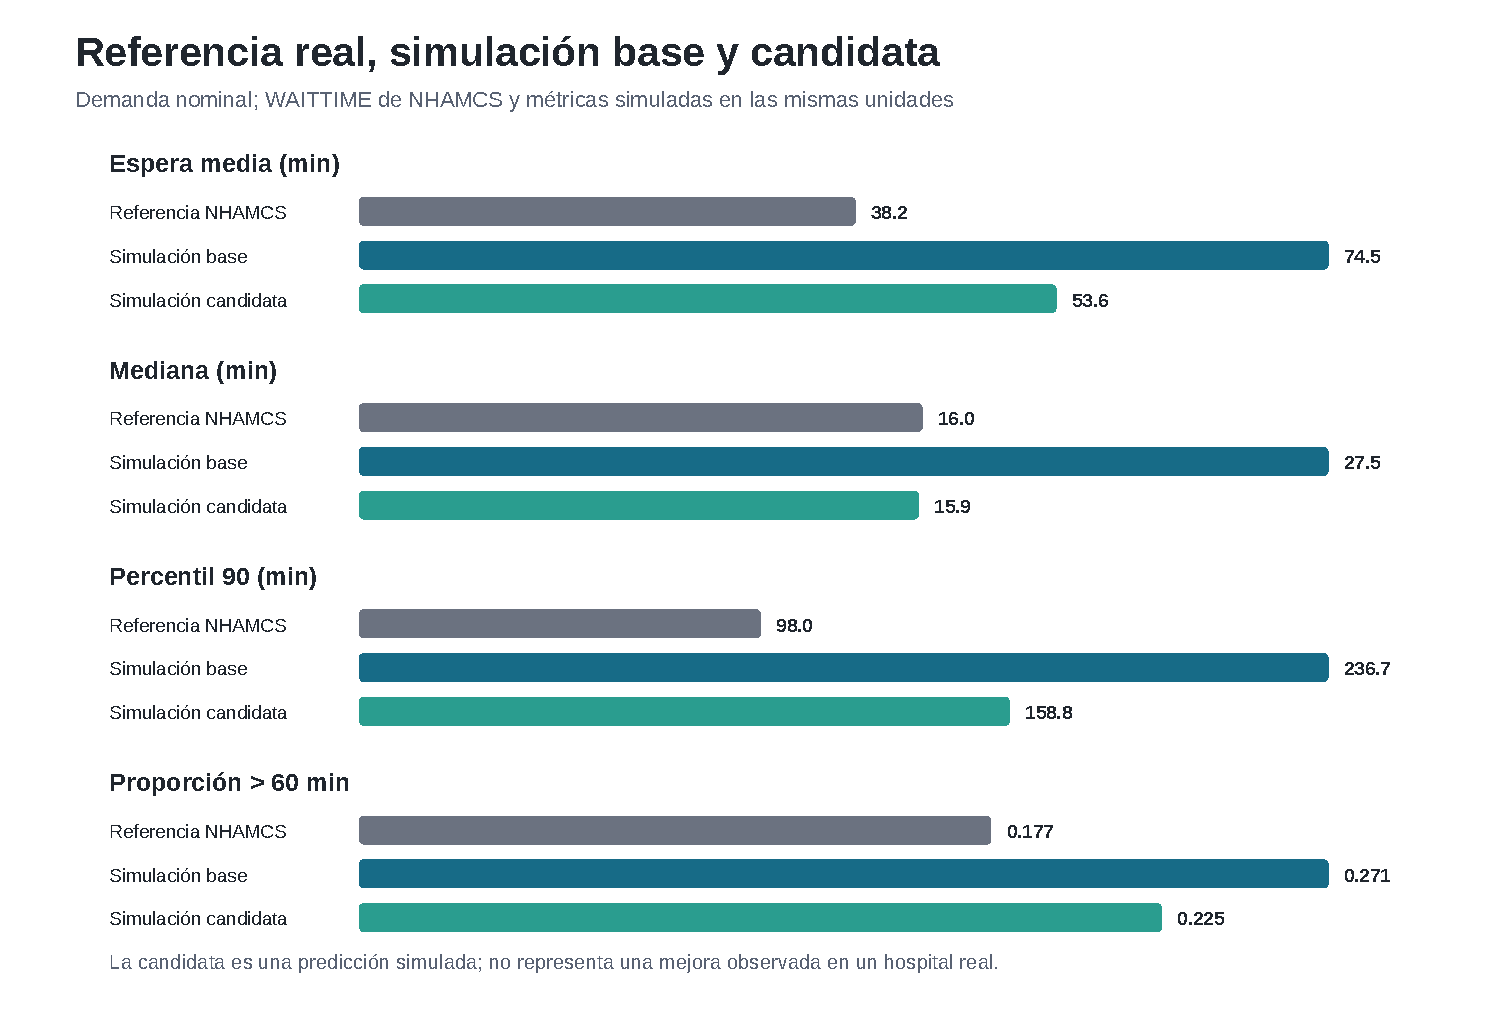
\includegraphics[width=0.92\linewidth]{figures/validation_comparison.pdf}
\caption{Comparación de la referencia NHAMCS 2022 con la simulación base y la candidata
(figura generada en \texttt{evidence/final/figures/}).}
\label{fig:validacion}
\end{figure}

\subsection{Interpretación}
\begin{itemize}
  \item El modelo base \textbf{sobreestima las cuatro métricas}: espera media de \WaitBaseNom{}
  frente a \RefMeanWait{} min (IC 95\,\% de la referencia [\RefMeanCILow, \RefMeanCIHigh]),
  y percentil 90 de \NomBasePninety{} frente a \RefPninetyWait{} min. Su MAE en minutos es
  \MaeBase{}; en la proporción, \MaePropBase{}.
  \item La candidata queda más cerca (MAE de \MaeCand{} min; \MaePropCand{} en la
  proporción). Su mediana (\NomCandMedian{} min) casi coincide con la referencia
  (\RefMedianWait{} min), pero el percentil 90 candidato sigue \PninetyCandErr{} min por
  encima de NHAMCS: el modelo reproduce peor la cola larga.
  \item Que la candidata se aproxime a la referencia \emph{no convierte la intervención en
  validada}: el algoritmo minimizó la espera simulada, no se ajustó a \texttt{WAITTIME}, y la
  referencia es el desempeño observado de departamentos heterogéneos, no el efecto de un
  cambio de horario.
\end{itemize}

\subsection{Límites de la comparación}
\texttt{WAITTIME} mide la espera hasta el primer contacto con médico, APRN o PA, mientras el
modelo mide la espera hasta que un equipo inicia la atención; las poblaciones también
difieren (promedio nacional de muchos DE frente a un DE sintético de volumen mediano). La
correspondencia del modelo es, por tanto, parcial. La discrepancia en la cola larga puede
deberse a un servicio supuesto demasiado largo, a la falta de variabilidad del proceso real
o a la diferencia de métrica; este informe no permite distinguir entre estas explicaciones.

\section{Resultados: base, mejora y sensibilidad}
\label{sec:resultados}

\begin{alcance}
Todo lo que sigue son resultados de \textbf{simulación} (\texttt{synthetic\_simulation}) con
parámetros calibrados con NHAMCS 2022 y un servicio supuesto. Describen una mejora
\emph{simulada}; no se observó ninguna mejora en un hospital.
\end{alcance}

\subsection{Condiciones y variabilidad}
La tabla~\ref{tab:condiciones} muestra la espera media de las seis condiciones con su
dispersión entre réplicas. La variación entre días simulados es grande: la desviación
estándar de la espera media nominal es \StdBaseNom{} min (base) y \StdCandNom{} min
(candidata), y los intervalos marginales del 95\,\% de la media
([\MargBaseLow, \MargBaseHigh] y [\MargCandLow, \MargCandHigh] min) se solapan. Por eso el
efecto del horario se estima con diferencias pareadas, que eliminan parte de la variación
compartida.

\begin{table}[ht]
\centering\small
\caption{Espera media por condición ($n=\NReps$ réplicas cada una). El drenaje es el tiempo
posterior al cierre de la ventana hasta que toda la cohorte medida inicia atención; no entra
en las métricas de cola ni de utilización.}
\label{tab:condiciones}
\fittable{generated/tab_conditions.tex}
\end{table}

\begin{figure}[ht]
\centering
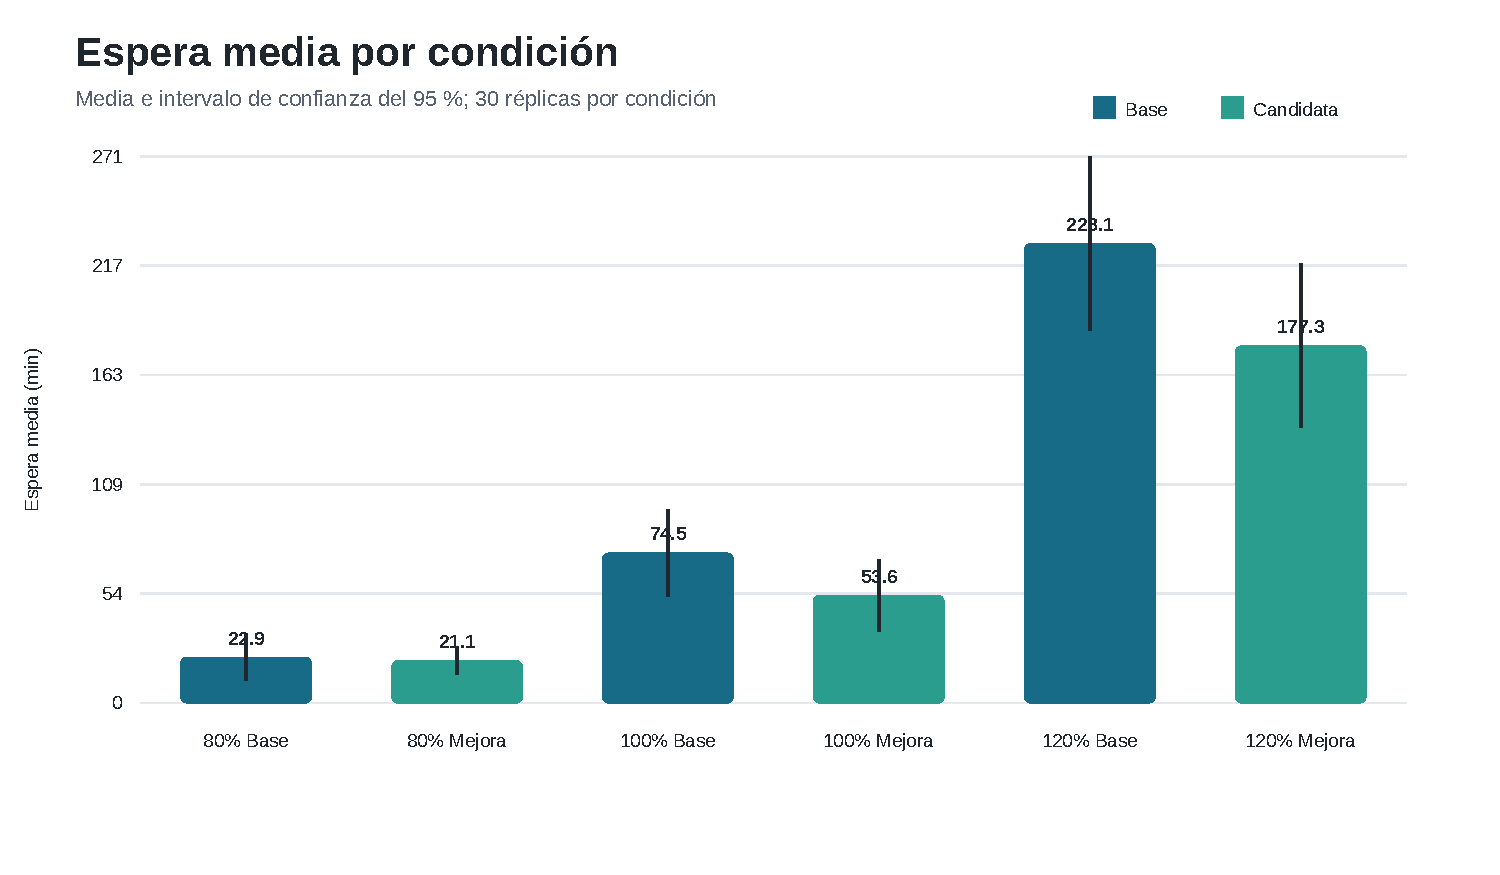
\includegraphics[width=0.92\linewidth]{figures/mean_wait_by_condition.pdf}
\caption{Espera media por condición, con intervalo de confianza del 95\,\% (30 réplicas por
condición). Figura generada en \texttt{evidence/final/figures/}.}
\label{fig:condiciones}
\end{figure}

\subsection{Efecto del horario sobre la espera media}
\begin{table}[ht]
\centering\small
\caption{Diferencia pareada de la espera media (base $-$ candidata). Valores positivos
indican menos espera con la candidata. El intervalo es normal del 95\,\% para la media de las
\NReps{} diferencias pareadas.}
\label{tab:pareada}
\fittable{generated/tab_paired_mean_wait.tex}
\end{table}

\begin{figure}[ht]
\centering
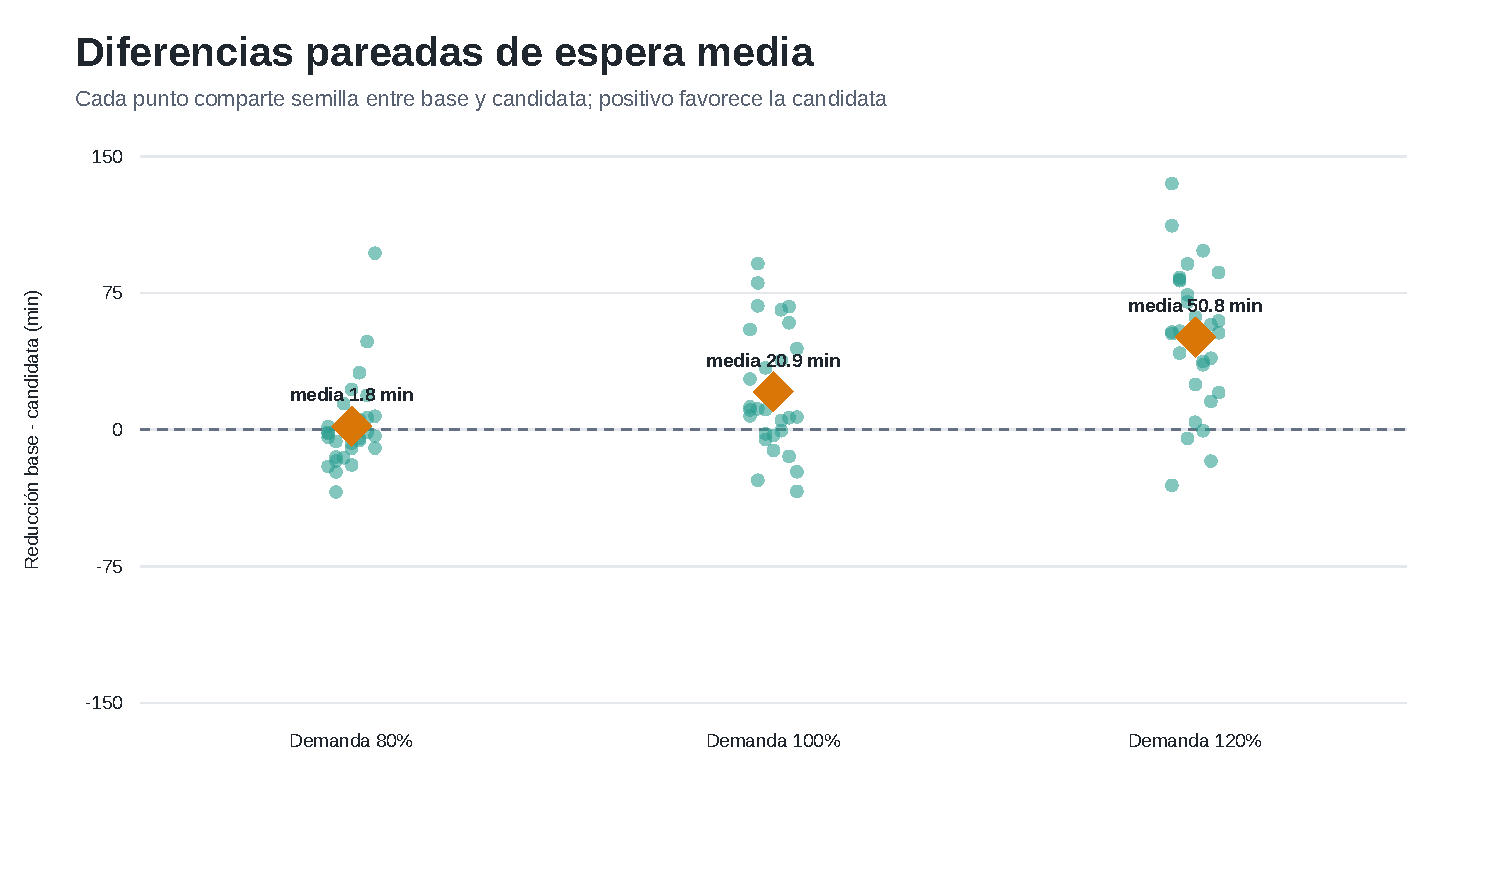
\includegraphics[width=0.92\linewidth]{figures/paired_wait_improvement.pdf}
\caption{Distribución de la mejora pareada de la espera media por nivel de demanda
(figura generada en \texttt{evidence/final/figures/}).}
\label{fig:pareada}
\end{figure}

La reducción es de \RedNom{} min (\RedPctNom\,\%) con demanda nominal y de \RedHigh{} min
(\RedPctHigh\,\%) con demanda alta; en ambos casos el intervalo pareado excluye el cero y la
candidata favorece a \PairsPosNom{} y a \PairsPosHigh{} de las \NReps{} parejas, respectivamente.
Con demanda baja la reducción media es de \RedLow{} min, el intervalo
([\RedCILowLow, \RedCIHighLow]) incluye el cero y solo \PairsPosLow{} de \NReps{} parejas
favorecen a la candidata: \textbf{no se afirma una mejora consistente} en esa condición.
El mayor efecto absoluto aparece cuando el sistema está más exigido.

\subsection{Otras métricas}
\begin{table}[ht]
\centering\small
\caption{Métricas bajo demanda nominal. El cambio es candidata $-$ base; el intervalo de la
última columna corresponde a la reducción pareada (base $-$ candidata).}
\label{tab:nominal}
\fittable{generated/tab_nominal.tex}
\end{table}

\begin{table}[ht]
\centering\small
\caption{Sensibilidad a la demanda del percentil 90, de la proporción con espera mayor a 60
minutos y de la cola media. Reducción = base $-$ candidata (intervalo pareado del 95\,\%).}
\label{tab:sensibilidad}
\fittable{generated/tab_secondary_by_demand.tex}
\end{table}

Con demanda nominal la candidata reduce también la mediana (\NomBaseMedian{} a
\NomCandMedian{} min), el percentil 90 (\NomBasePninety{} a \NomCandPninety{} min), la
proporción con espera mayor a 60 minutos (\NomBaseShare{} a \NomCandShare{}) y la cola media
(\NomBaseQueue{} a \NomCandQueue{} pacientes). El resultado no se obtiene con más recursos: ambos
horarios usan 23 unidades. La utilización efectiva de la candidata es ligeramente menor, lo
que refleja una mejor coincidencia temporal entre demanda y capacidad, no capacidad adicional.

\subsection{Congestión terminal}
El drenaje medio tras el cierre de la ventana es de \DrainBaseNom{} min en la base y
\DrainCandNom{} min en la candidata bajo demanda nominal, y sube a \DrainBaseHigh{} y
\DrainCandHigh{} min con demanda alta. Las esperas se reportan completas (sin censura), pero
esos drenajes prolongados muestran saturación y limitan la extrapolación de la condición
de demanda alta.

\section{Incertidumbre, limitaciones y amenazas a la validez}
\label{sec:incertidumbre}

\subsection{Incertidumbre cuantificada}
La incertidumbre que sí se mide es la del muestreo de la simulación: desviaciones estándar
entre réplicas, intervalos normales del 95\,\% para las medias y para las diferencias
pareadas, y el número de parejas favorables. Con \NReps{} réplicas los intervalos son
amplios (por ejemplo, [\RedCILowNom, \RedCIHighNom] min para la reducción nominal). La
distribución de la espera es sesgada y con colas largas, por lo que el intervalo normal es
solo una aproximación; no se ejecutaron pruebas de normalidad, \emph{bootstrap} ni pruebas
de hipótesis.

\subsection{Incertidumbre no cuantificada}
\begin{itemize}
  \item \textbf{Parámetros de servicio.} Medianas y $\sigma$ son supuestos; el estudio no
  propaga su incertidumbre. Es la entrada con más influencia potencial sobre la congestión y
  la principal amenaza a la validez. El proxy de \texttt{LOV} las acota por arriba, pero no
  las identifica.
  \item \textbf{Una sola referencia de volumen.} Solo se usa el DE de volumen mediano; el
  resultado depende del nivel de utilización. La sensibilidad a la demanda
  (0.80--1.20) cubre parcialmente esta dependencia.
  \item \textbf{Sensibilidad no explorada.} No se varió el presupuesto de recursos, los
  pesos de la función objetivo, la penalización de censura ni la distribución de servicio.
  \item \textbf{Sin comparador de optimización.} No hay búsqueda aleatoria con el mismo
  presupuesto de evaluaciones; no se sabe cuánto aporta la estructura del GA, ni si hay
  horarios factibles mejores que la candidata.
\end{itemize}

\subsection{Limitaciones del modelo y de la referencia}
\begin{itemize}
  \item Recurso único agregado: no modela médicos, enfermería, diagnóstico ni camas por
  separado, ni preempción, abandono, reingresos o etapas múltiples.
  \item Tasa constante por hora y un solo día de medición por réplica; no se modelan
  variaciones por día de la semana, estación o crisis.
  \item NHAMCS es una muestra nacional de Estados Unidos, con no respuesta alta en
  \texttt{IMMEDR} y \texttt{WAITTIME}; su perfil agregado mezcla DE de distintos tamaños.
  \item El volumen por DE se aproxima como $\sum \texttt{PATWT}/\texttt{EDWT}$ con 188 DE.
  \item Los cuantiles de la referencia no tienen error estándar y el criterio de
  fiabilidad es una versión simplificada del de NCHS \citep{parker2017standards}.
\end{itemize}

\subsection{Sobreajuste de la candidata}
La mejora medida en el conjunto de optimización (\OptRelPct\,\% en el objetivo) es mayor
que la medida con semillas independientes (\RedPctNom\,\% en la espera media). Es el
comportamiento esperable cuando se elige el mejor entre varios horarios sobre un mismo
conjunto de semillas, y es la razón de reportar solo la evaluación independiente.

\subsection{Riesgo de extrapolación}
Los resultados aplican solo a las distribuciones, volumen, capacidad y horizonte probados.
No cubren crisis, cambios clínicos, abandono, preempción, etapas múltiples de atención ni un
hospital particular. En demanda alta el sistema se satura (sección~\ref{sec:resultados}) y la
cifra de mejora de esa condición debe leerse como indicativa. Para trasladar el análisis a
un hospital concreto harían falta datos locales de llegadas, triaje, capacidad y tiempo de
ocupación del equipo, una calibración propia del servicio y una validación externa.

\section{Conclusiones y recomendación}

\textbf{Qué mejoró.} Bajo los supuestos del modelo, redistribuir las mismas 23 unidades de
capacidad con el horario candidato (1, 2, 5, 5, 6, 4) reduce la espera hasta el inicio de la
atención respecto del horario base (3, 3, 4, 4, 5, 4).

\textbf{Cuánto.} Con demanda nominal, la espera media simulada baja de \WaitBaseNom{} a
\WaitCandNom{} min (reducción pareada de \RedNom{} min, \RedPctNom\,\%; IC 95\,\%
[\RedCILowNom, \RedCIHighNom] min), y también bajan la mediana, el percentil 90, la
proporción con espera mayor a 60 minutos y la cola.

\textbf{Bajo qué condiciones.} El efecto depende de la carga: con demanda alta la
reducción absoluta es mayor (\RedHigh{} min), y con demanda baja no se distingue de cero
(IC 95\,\% [\RedCILowLow, \RedCIHighLow] min). La mejora es consistente solo cuando el
sistema está lo bastante exigido.

\textbf{Qué tan confiable es la comparación.} La comparación entre horarios es pareada, con
semillas independientes de las de optimización y \NReps{} réplicas por condición, pero la
variabilidad entre días es alta. La validación frente a NHAMCS es parcial: el modelo base
sobreestima la espera observada (MAE de \MaeBase{} min en la base y de \MaeCand{} min en la
candidata), por lo que las cifras absolutas de espera no deben tomarse como predicciones.
Con más confianza se puede leer la \emph{dirección} del efecto que su magnitud.

\textbf{Qué limitaciones permanecen.} El servicio es un supuesto; no hay comparador de
optimización ni sensibilidad a los parámetros del GA y del servicio; el modelo es un recurso
agregado calibrado con un DE nacional estadounidense, no con un hospital guatemalteco.

\textbf{Recomendación.} Conservar la candidata como escenario de análisis y demostración,
no como política lista para aplicar. Como pasos siguientes, en orden de prioridad:
(1)~calibrar el servicio con datos de ocupación del equipo (o al menos propagar la
incertidumbre del supuesto con un análisis de sensibilidad); (2)~añadir una búsqueda
aleatoria con el mismo presupuesto para medir el aporte del GA; (3)~ampliar la
sensibilidad a demanda, presupuesto y pesos del objetivo; (4)~validar con datos locales
antes de cualquier decisión operativa.

\begin{alcance}
La conclusión es sobre una \textbf{mejora simulada} bajo supuestos explícitos y una
referencia pública de Estados Unidos. No demuestra causalidad ni una mejora clínica real.
\end{alcance}

\section{Contribuciones, uso de inteligencia artificial y reproducibilidad}

\subsection{Contribuciones}
La tabla resume el registro final de \texttt{docs/contributions.md}. Cada aporte se
vincula con archivos, pruebas, resultados o materiales verificables del repositorio.

\begin{table}[ht]
\centering\small
\caption{Registro de contribuciones.}
\label{tab:contribuciones}
\begin{tabularx}{\linewidth}{@{}l X@{}}
\toprule
Integrante & Contribución registrada \\
\midrule
Pablo Daniel Barillas Moreno & Coordinación e integración; definición del problema; investigación del algoritmo genético; implementación inicial del simulador, la CLI y la optimización restringida; reproducibilidad y cierre \\
Jorge Palacios & Pipeline reproducible de NHAMCS 2022 (descarga, preparación, calibración y pruebas), agregados en \texttt{data/processed/}, \texttt{docs/05\_data\_calibration.md} y entradas NHAMCS de la bibliografía \\
Adrián Ricardo González Muralles & Correcciones del simulador (cola tras calentamiento, drenaje, capacidad efectiva), diseño factorial, candidata congelada, 180 ejecuciones, validación frente a NHAMCS, figuras y pruebas \\
Andrés Rafael Chivalán & Interfaz Streamlit en cinco páginas, formularios de ejecución controlada, visualizaciones, evidencia precomputada, descargas y pruebas de interfaz \\
Javier Andrés Chen & Informe técnico en LaTeX, generación reproducible de tablas y figuras (\texttt{Output/report/}, \texttt{Output/scripts/build\_report\_assets.py}), presentación y guion cronometrado \\
\bottomrule
\end{tabularx}
\end{table}

\subsection{Uso de inteligencia artificial}
Se declara en \texttt{docs/ai\_usage.md}: OpenAI Codex apoyó la planificación, la estructura
del repositorio, la revisión de código, las correcciones del simulador, el pipeline
experimental y la documentación inicial; Claude Code apoyó la documentación del pipeline de
calibración de NHAMCS. Para este informe se usó además Claude (Anthropic) como apoyo para
estructurar y redactar el borrador y para escribir el script que convierte la evidencia en
tablas y figuras. Las cifras proceden exclusivamente de \texttt{evidence/final/} y de
\texttt{data/processed/}, y los integrantes son responsables de revisarlas y de poder
explicarlas. Las herramientas de IA no se usaron como fuente de datos ni como autoridad
bibliográfica.

\subsection{Reproducibilidad del informe}
Las tablas, las macros con cifras y las figuras de este informe se regeneran con
\begin{center}\small\texttt{python Output/scripts/build\_report\_assets.py}\end{center}
y el documento se compila con \texttt{latexmk -xelatex main.tex} desde
\texttt{Output/report/}.
Ninguna cifra de las secciones de resultados se escribió a mano.


\bibliographystyle{plainnat}
\bibliography{references}

\end{document}
